\documentclass{article}

% if you need to pass options to natbib, use, e.g.:
    \PassOptionsToPackage{numbers, compress}{natbib}
% before loading neurips_2020

% ready for submission
% \usepackage{neurips_2020}

% to compile a preprint version, e.g., for submission to arXiv, add add the
% [preprint] option:
    \usepackage[preprint]{neurips_2020}

% to compile a camera-ready version, add the [final] option, e.g.:
    % \usepackage[final]{neurips_2020}

% to avoid loading the natbib package, add option nonatbib:
    %  \usepackage[nonatbib]{neurips_2020}

\usepackage[utf8]{inputenc} % allow utf-8 input
\usepackage[T1]{fontenc}    % use 8-bit T1 fonts
\usepackage{hyperref}       % hyperlinks
\usepackage{url}            % simple URL typesetting
\usepackage{booktabs}       % professional-quality tables
\usepackage{amsfonts}       % blackboard math symbols
\usepackage{nicefrac}       % compact symbols for 1/2, etc.
\usepackage{microtype}      % microtypography
\usepackage{xcolor}
\usepackage[pdftex]{graphicx}

\title{Machine Learning Enhancements to Particle Physics Simulations to Reduce Computational Complexity}

% The \author macro works with any number of authors. There are two commands
% used to separate the names and addresses of multiple authors: \And and \AND.
% Using \And between authors leaves it to LaTeX to determine where to break the
% lines. Using \AND forces a line break at that point. So, if LaTeX puts 3 of 4
% authors names on the first line, and the last on the second line, try using
% \AND instead of \And before the third author name.

\author{%
  Robert Johnston \quad Patrick Moran \quad Sangbaek Lee   \\
  Laboratory for Nuclear Science\\
  Massachusetts Institute of Technology\\
  Cambridge, MA 02139 \\
  \texttt{\{robertej, moranp, sangbaek\}@mit.edu} \\
  % examples of more authors
  % \AND
  % Coauthor \\
  % Affiliation \\
  % Address \\
  % \texttt{email} \\
  % \And
  % Coauthor \\
  % Affiliation \\
  % Address \\
  % \texttt{email} \\
  % \And
  % Coauthor \\
  % Affiliation \\
  % Address \\
  % \texttt{email} \\
}

\begin{document}

\maketitle

%%\begin{abstract}
		%Pat's original email
		%In our experiment (CLAS12 at Jefferson Lab), we have event generators that simulate a large number of particle physics events, each of which consist of a number of kinematic variables.
		%The output of these event generators are then passed to another simulation framework that simulates these generated events in the detector geometry of the experiment. 
		%This latter process is very time-consuming given the large number of events that we want to reconstruct in our detectors.
		%We would like to develop a machine learning project that can train on the generated events and reconstructed events, and then predict the output of reconstruction based on the kinematic variables of the generated event.
		%This would allow us to reconstruct only a small amount of generated events through the reconstruction framework, thus drastically reducing the computing time needed for our research.
%% 		An electron-proton scattering experiment has been performed in the CLAS12 detector at the Thomas Jefferson National Accelerator Facility in order to probe the three-dimensional structure of the proton.
%%         Yields of scattered particles into the detector are determined by the types of interactions between incoming electrons and stationary protons.
%%         To understand the underlying physical processes observed in the experiment, the detector acceptance, which is the ratio of the number of events that are detected to the number that are produced, should be precisely estimated. 
%% 		The traditional method is to generate simulated data describing physical processes based on existing knowledge, then to pass these events to the Geant4 software package to simulate their interactions in the detector material.
%% 		A novel method to predict the output of reconstruction based on the kinematic variables of the generated events is described in this project.
%% 		This work is expected to drastically reduce the computing time needed for detector acceptance studies.
%%\end{abstract}


% Evaluation metrics for project proposal (10 points)
% Previous work and references: 2 points
% Understanding the problem, it’s formulation, and goal: 2 points
% Dataset to be used or collected, method or algorithm proposed: 2 points
% Well defined evaluation criteria: 2 points
% Writing clarity and structure: 2 points

% Questions you may answer when writing your proposal:
% What do you want to do? What question are you answering?
% What data will you use? Give a specific description of the data
% and confirm that you already have the data in hand at this point.
% What is your motivation? Formulate your problem as a machine learning problem.
% What methods will you try and compare?
% What computational resources will you use? Think about time and feasibility.
% Relevant related work? (brief summary)
% What is your project plan? You may include key steps and rough internal deadlines for each step.
% What are the risks? What might turn out to be more difficult than you anticipated? And how might you mitigate these risks?

\section{Proposal}
% What do you want to do? What question are you answering?
\quad In an electron-proton scattering experiment in the CLAS12 detector at Thomas Jefferson National Accelerator Facility (JLab) [\citet{BURKERT2020163419}], an incoming electron beam near the speed of light is incident on a stationary proton target. The electron and proton interact and can produce final state particles according to the governing physical laws that include quantum field theory. The particle species of incoming particles and products are called initial and final states, respectively. For each DVEP, the final states are uniquely determined. For example, one DVEP, called Deeply Virtual $\pi^0$ Production (DV$\pi^0$P), has one electron, one proton, and two photons as its final state [\citet{PhysRevD.55.7114}].

% What data will you use? Give a specific description of the data
% and confirm that you already have the data in hand at this point.
\quad An event is defined as a set of particles detected in the interaction time scale. One widely accepted way of analyzing events is to compare experimental results with Monte-Carlo simulated data set [\citet{PhysRevLett.115.212003, 10.1093/ptep/ptaa104}]. The standard simulation consists of two steps. First, we generate a data set of particle momenta based on prior knowledge before particles pass the detectors. Second, the second step is to pass these events to the GEANT4 package [\citet{AGOSTINELLI2003250}], which simulates the interaction between the final states and detectors. This serial simulation can be performed using computing facilities connected to Open Science Grid (OSG), including MIT farms. The simulated data of a few million events are already achieved, more amounts of simulated data can be easily taken from OSG. For example, in one day, we can roughly simulate 100M events of data.

% What is your motivation? Formulate your problem as a machine learning problem.
\quad Before we discuss the machine learning techniques, we start from a toy model, a baseball game with one pitcher and one catcher. In one "inning", the pitcher throws a ball four times in a row, knowing the ball's velocity and direction in spherical coordinates (velocity, polar angle $\theta$, azimuthal angle $\phi$) in the beginning. In $i$-th inning, the pitcher has the data $z^{i}$ as 4$\times$3 matrices. The catcher also records the four ball's velocities and directions in $x^{i}$'s in 4$\times$3 matrices. The first two innings are visualized in Fig.~\ref{data}-a. The catcher may catch all of the balls correctly like $x^0$, and sometimes miss some balls like $x^1$. One wants to collect the pair of $z^i$ and $x^i$, but notices that hiring a catcher is way more expensive than hiring a pitcher.

\begin{figure}[!hb]
 \centering
   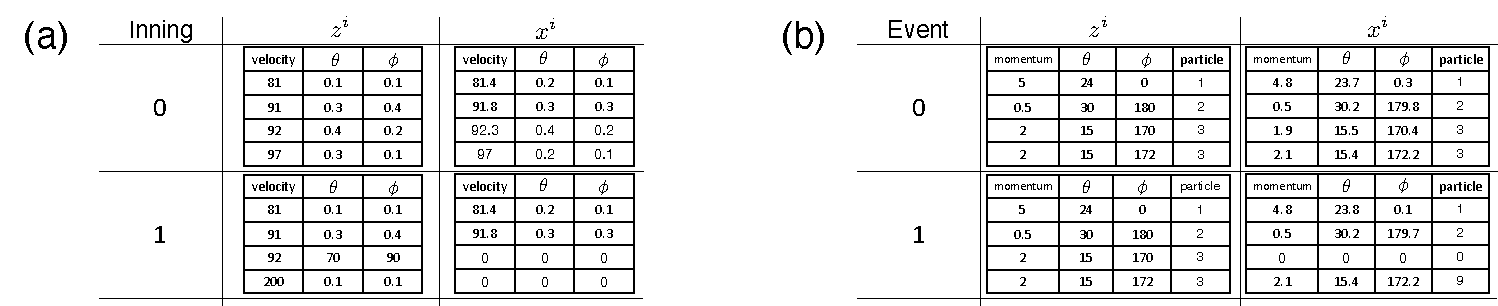
\includegraphics[width=\linewidth]{dataDescription.pdf}
  \caption{The first two rows of (a) toy model data with a pitcher and a catcher, (b) actual data with particles.}
  \label{data}
\end{figure}

\quad In our simulated data, the pitcher's record $z^i$ corresponds to the results of step 1 of the serial simulation, and the catcher's record $x^i$ corresponds to the results of step 2 simulation. The results of each simulation can be encoded as particle's kinematic information. One particle has 4 dimensional information, where 3 dimensions come from (momentum, polar angle $\theta$, azimutha angle $\phi$) and another one from particle species. The example of the first two events are in Fig.~\ref{data}-b. In summary, $x^i$'s are in \{4$\times$4\}$\times d$, and $z^i$'s are also in \{4$\times$4\}$\times d$ dimension, when $d$ is total number of events. From our experiences, for one day simulation, only 10 minutes are spent to simulate $z^i$, while the rest of time spent is attributed to simulate $x^i$.

% What methods will you try and compare?
\quad Given the motivation, we aim to replace step 2 simulation with some generative models that takes input as $z^i$, and output as $x^i$. We propose the normalizing flow (NF) [\citet{9089305, papamakarios2019normalizing}] as our generative model. \textcolor{red}{need details.}

% Relevant related work? (brief summary)
related work: \citet{PhysRevD.101.076002}\textcolor{red}{need details.}



% What computational resources will you use? Think about time and feasibility.
\quad We, as members of the MIT Hadronic Physics group, are granted access to MIT clusters such as an HTCondor farm, LHC Tier-2 \footnote{monitored at \url{http://www.cmsaf.mit.edu/condor4web/}}, and a slurm farm, EAPS cluster. Some farms external to MIT can be accessed using OSG for CLAS12 collaboration. The ifarm also offers some computing power \footnote{monitored at \url{https://scicomp.jlab.org/scicomp/index.html\#/farmJobs/activeJob}}. These farms are operating anytime. Especially, EAPS cluster runs without any delay, and supports disk space of 2 TB quota. The experimental data in interest is smaller than 100 GB, and simulated data takes roughly 400 MB for 5M events.


% What is your project plan? You may include key steps and rough internal deadlines for each step.
\begin{center}
\textbf{Proposed Project Timeline}\\~\\
\begin{tabular}{ c c c }
%\textbf{Date} & \textbf{Project Milestone} \\ 
  \textbf{March 31} & Decide on optimal ML method for this project \\
  \textbf{April 10} & Have minimal working example on small dataset  \\  
  \textbf{April 25} & Have working example on full scope of problem \\ 
  \textbf{May 4} & Conclude production run of project, begin finalizing reports
\end{tabular}
\end{center}

% What are the risks? What might turn out to be more difficult than you anticipated? And how might you mitigate these risks?
\quad \textcolor{red}{do we want to change this part too?}The overarching goal of this project is to provide a correction factor for detector acceptance in our experiment. This will be a large, overall normalization factor, and as our thesis goal is to measure absolute quantities (rather than ratios) this project runs the risk of providing an inaccurate acceptance correction term, which would then yield a significantly shifted final result. This can be mitigated by extensive cross-validation of results, and can be extensively verified by running large simulations in a small region of phase space to create new data for comparison purposes.

\quad \textcolor{red}{do we want to change this part too?}On a more technical level, as this is a very high dimensional problem, it could be difficult to engineer an efficient algorithm for this process. This issue could be mitigated by building up to our actual process in incremental steps, e.g., trying to build an algorithm that will be able to efficiently predict the outcome of just one simulated particle, and then build onto more complex initial and final states. If we are not able to realize our full initial and final state mappings to yield correction factors, we would still be able to gain useful insight by understanding better how single particles, e.g. electrons, traverse through our detector. 



%garbages previously submitted
%Since the experimental discovery of the proton by Ernest Rutherford over 100 years ago, there have been various attempts to reveal its internal structure. Yet, its three dimensional profile is still elusive. Measurements on deeply virtual exclusive processes (DVEP) from electron-proton scattering are one proposed way to project the proton structure [\citet{PhysRevD.55.7114}]. In the CLAS12 detector at Thomas Jefferson National Accelerator Facility (JLab), experimental data has been taken of these and other processes [\citet{BURKERT2020163419}].

%Ideally, an event should consist of initial and final states. This is not always true because particles in final states are stochastically detected, depending on their kinematics and detector efficiencies.

 %In this work, we match events $x^i$'s into binary labels $y^i$'s: (\textit{A}) events where every particle gets detected and is correctly classified as the final state of the exclusive process of interest; (\textit{B}) events that fail to be classified as the final state but come from the exclusive process. The goal of this work is to estimate the detector acceptance, the number of \textit{B} events based on measurements of \textit{A} events.  %; and (\textit{C}) events that are not related to the exclusive processes. 
 
 %commented by Sangbaek
 %In the real experiment, the number of events labelled as \textit{A} can be measured. On the other hand, it is hard to estimate the number of events labelled as \textit{B} from the experiment. One widely accepted way is to use a Monte-Carlo simulated data set to estimate the detector acceptance [\citet{PhysRevLett.115.212003, 10.1093/ptep/ptaa104}]. The simulation consists of two steps. The first step is to generate physical events by the Metropolis-Hastings algorithm. The second step is to pass these events to the GEANT4 package [\citet{AGOSTINELLI2003250}], which simulates the interaction between the final states and detectors. The experimental data is stored in the JLab computing facility, which can be accessed by ssh-ing into their farm, named ifarm. Simulated data can also be achieved using computing facilities connected to Open Science Grid (OSG), including MIT farms. The simulated data of a few million events are already achieved, more amounts of simulated data can be easily taken from OSG. For example, in one day, we can roughly simulate 100M events of data.


%Unlike our physics process of interest, which has a high dimensional phase space, most physics final states are considerably more simple, and as such, it has been easier for previous experiments to just run GEANT4 simulations, rather than use machine learning to determine acceptance corrections. As such, work exactly similar to our proposed project has not yet been performed, but machine learning techniques are ubiquitous throughout our research community. Convolutional neural networks (CNN) have been explored by the ALICE collaboration at CERN to supplement particle identification algorithms [\citet{Viljoen2020}], essentially analogous to our project except we will classify whole events, rather than individual particles. Moreover, research is ongoing with replacing traditional GEANT4 simulations with ML boosting to produce 'fast simulations' wherein computationally expensive simulation over dense detector materials are replaced with GANs and VAEs to yield orders of magnitude speedup in simulation time [\citet{Albertsson2018}, \citet{Paganini2017}].


%There are difficulties in estimating the detector acceptance using simulated data. Generally, this type of computing takes too much time to collect significant statistics. Also, sometimes kinematics of label \textit{A} events in simulation may not match with label \textit{A} events in the real experiment. Also, the ratio from simulated data largely depends on theoretical model for probability distribution that was used for Metropolis-Hastings algorithm. Finally, the acceptance only depends on particle kinematics, so it is not efficient to run each process for large statistics. Now this task can be re-defined as a machine learning problem in following way. We have particle momenta in the experimental and simulated data. As indicated earlier, the detector acceptance, despite being stochastic, must be a function of momenta of final states. We take momenta of final states as feature vectors. Each event has label of detector acceptance $\in$ [0, 1], by definition. We define training data sets as simulated data, and a test data set as experimental data. We keep cross validate with several training data sets, and apply our algorithm to the test data.

%Like previous works, we propose using CNN and GAN for this project. First, we will try regression with CNN with simulated data, and test on experimental data. Second, we will try GAN to mimic our simulated data to get more statistics without performing more simulation. We will estimate the detector acceptance with GAN data, and compare the detector acceptance for the experimental data.

\newpage
\small
\bibliographystyle{unsrtnat}
\bibliography{references}
% [1] Alexander, J.A.\ \& Mozer, M.C.\ (1995) Template-based algorithms for
% connectionist rule extraction. In G.\ Tesauro, D.S.\ Touretzky and T.K.\ Leen
% (eds.), {\it Advances in Neural Information Processing Systems 7},
% pp.\ 609--616. Cambridge, MA: MIT Press.

% [2] Bower, J.M.\ \& Beeman, D.\ (1995) {\it The Book of GENESIS: Exploring
%   Realistic Neural Models with the GEneral NEural SImulation System.}  New York:
% TELOS/Springer--Verlag.

% [3] Hasselmo, M.E., Schnell, E.\ \& Barkai, E.\ (1995) Dynamics of learning and
% recall at excitatory recurrent synapses and cholinergic modulation in rat
% hippocampal region CA3. {\it Journal of Neuroscience} {\bf 15}(7):5249-5262.

\end{document}